\documentclass[paper-main.tex]{subfiles}

\begin{document}



\section{Open-source code}
\label{app:code}
This project was implemented in python3~\cite{python} scripts as well as jupyter notebooks~\cite{jupyter}~\cite{ipython} and used the packages of numpy~\cite{numpy}, scipy~\cite{scipy}, matplotlib~\cite{matplotlib}, tqdm~\cite{tqdm}, and logmmse~\cite{logmmse}.

The current build and sample recordings of the optical microphone can be found at:
\url{https://github.com/daccordeon/gravexplain}
% \begin{verbatim}
% README
% \end{verbatim}

\section{Implementation of the Viterbi algorithm}
\label{app:viterbi}

We used the Viterbi algorithm to find a signal in a spectrogram. Here we detail the implementation used.

We consider a spectrogram grid where each element in the grid is the Fourier amplitude of a particular frequency at a particular time. These are normalised between $(0, 1)$ to use as multiplicative weights. In fact, we take the logarithm and so the sum of all weights to avoid underflow. The best path has the highest weight among all paths.

With the grid prepared, the algorithm starts in the second column. In each iteration, the algorithm looks for the best path to each cell from the cells in the previous column, selecting the previous cell with the greatest cumulative weight among those ‘nearby’ (the value of which was discovered in the previous iteration). Where the cumulative weight is the weight of the best path to reach that previous cell. The nearness of a previous cell is given by the limit on the allowed frequency change over time.

For each cell in the current column, the algorithm calculates the cumulative weight to reach that cell by adding its weight to the cumulative weight to reach it. The algorithm also notes the row index of which cell in the previous column it best connects to.
Continuing like this until it reaches the end of the grid, the algorithm then looks for the greatest weight in the last column and retraces the indices of the steps it took until it reaches the start of the grid. That discovered best path is the Viterbi path.


\section{A common mistake for those new to wandering frequency signals}
\label{app:phase_gotcha}

We want to generate a sine wave that changes frequency over time so that the frequency at some time is given by a function $f(t)$. A common mistake is to appeal to the standard form $\sin{(2 \pi f t)}$, where f is a constant frequency, and guess $\sin{(2 \pi f(t) t)}$. However, this fails to address the phase accumulated earlier in the signal. Instead, the standard form in fact says that for some $\sin{(F(t))}$ it is true that $\frac{dF}{dt}(t) = 2 \pi f(t)$, where $f(t)$ gives the frequency of $\sin{(F(t))}$ at time $t$. Therefore, the correct form for a wandering tone is $\sin{(\int{2 \pi f(t) dt})}$.
% This formula is also useful when performing frequency modulation.


\section{Photodiode circuit design}
\label{app:circuit_diagram}
% schematic of breadboard and connections to pi
% https://www.circuit-diagram.org/editor/
% https://crcit.net/c/e397dcc2166943d69155f9dac1e27bce

Figure~\ref{fig:circuit_diagram} shows the photodiode circuit diagram, it is also available at \url{https://crcit.net/c/e397dcc2166943d69155f9dac1e27bce}. A photo of the breadboard and Raspberry Pi pins is shown in Figure~\ref{fig:circuit_pic3}. This design was based off standard examples of photo-detectors, connecting an ADC to a Pi, and Sallen-Key filters.

\begin{figure*}
	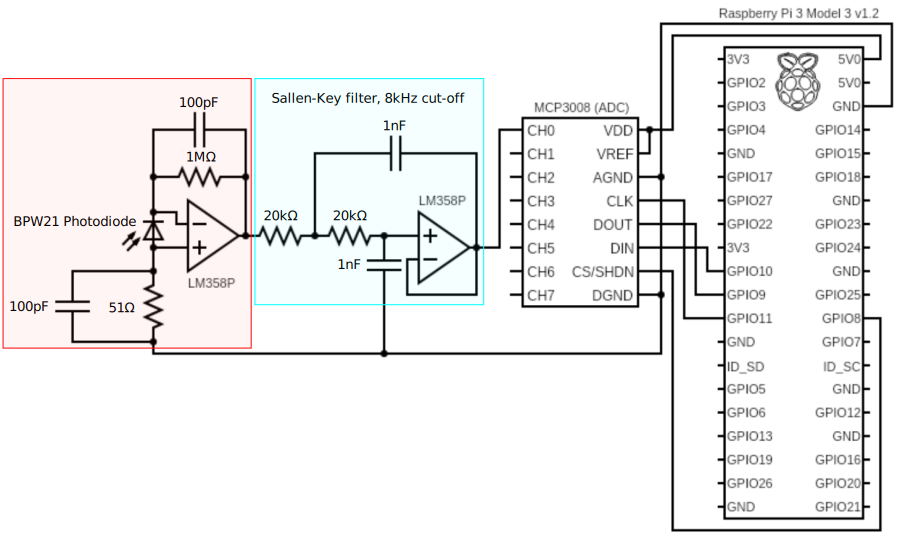
\includegraphics[width=.65\textwidth]{figures/circuit_diagram_2.pdf}
	\caption{Circuit diagram for photodiode reading. Photodiode in reverse-bias over an op-amp, analog signal then passed through Sallen-Key anti-aliasing filter tuned to 16kHz, then into an analog-to-digital converter (ADC). The digitised signal is then read by the special purpose input (SPI) pins of a Raspberry Pi in standard configuration.}
	\label{fig:circuit_diagram}
\end{figure*}

\begin{figure*}%[H]
	\includegraphics[width=0.5\textwidth]{figures/circuit_pic3.pdf}
	\caption{Photo of photodiode circuit assembled on breadboard.}
	\label{fig:circuit_pic3}
\end{figure*}

\section{Interferometric intensity relation derivation}
\label{app:intensity_derivation}

To obtain part of the transfer function for the optical microphone, we want to know the resultant change in intensity, $\delta I$, at a point in the interference pattern, given a small change, $\delta d$, in the difference between the arm lengths of the mirrors. Let the point be at angle $\theta$ on the screen (in the far-field) above the central ray as measured from the mirrors. Noting circular symmetry as to not specify exactly where in the fringe the point is.

At this point, two rays meet, one from each mirror, with total electric field amplitude $E_1(t) + E_2(t)$. Given an initial difference between the arm lengths of $d$, the path difference between the two beams at the screen is $2 d \cos{\theta}$ as the longer beam must travel back and forth over the extra distance, and both travel at angle $\theta$ to meet the point~\cite{fringes:online}.

The intensity at the point is then the norm squared of the total electric field amplitude as expressed in Equation~\ref{eq:intensity_derivation} below.

\begin{align}
    E_1(t) &= A e^{i (k L - \omega t)} \\
    E_2(t) &= A e^{i (k (L + 2 d \cos{\theta}) - \omega t)} \\
    I(t) &= \lvert A e^{i (k L - \omega t)} + A e^{i (k (L + 2 d \cos{\theta}) - \omega t)} \rvert^2
\label{eq:intensity_derivation}    
\end{align}

Collapse the phase difference to some value $\phi = 2 k d \cos{\theta}$. Then expand the norm squared using Euler’s relation, $e^{i \theta} = \cos{\theta} + i \sin{\theta}$. Here we stop considering intensity as a function of time as the time dependence will vanish.

\begin{align}    
    I =& A^2 \lvert e^{i (k L - \omega t)} + e^{i (k L + \phi - \omega t)} \rvert^2,\, \phi = 2 k d \cos{\theta} \\
    I =& A^2 ((\cos{(k L - \omega t)} + \cos{(k L + \phi - \omega t)})^2 \nonumber\\ &+ (\sin{(k L - \omega t)} + \sin{(k L + \phi - \omega t)})^2)
\end{align}

Expand and collect like terms, pull out a factor of two, and then recognise the form of $\cos{(\alpha-\beta)}$.

\begin{align}
    I =& A^2 (1 + 2 \cos{(k L - \omega t)} \cos{(k L + \phi - \omega t)} \nonumber\\&+ 1 + 2 \sin{(k L - \omega t)} \sin{(k L + \phi - \omega t)}) \\
    I =& 2 A^2 (1 + \cos{\phi}),\, \phi = \frac{4 \pi d \cos{\theta}}{\lambda}
\end{align}

Finally, changing derivatives and expand $\phi$ to find that the change in intensity given a change in distance is non-linear, that ${\delta I}/{\delta d}$ is non-constant.

\begin{align}    
    \frac{\delta I}{\delta d} &= \frac{\delta I}{\delta \phi}\; \frac{\delta \phi}{\delta d}\\
    \frac{\delta I}{\delta\phi} &= - 2 A^2 \sin{\phi}\\
    \frac{\delta\phi}{\delta d} &= \frac{4 \pi \cos{\theta}}{\lambda}\\
    \therefore \frac{\delta I}{\delta d} &= \frac{- 8 \pi A^2 \cos{\theta}}{\lambda} \sin{(\frac{4 \pi \cos{\theta}}{\lambda} d)}
\end{align}

This non-linearity in part of the transfer function will make the reverse problem of extracting the original signal more difficult.





\end{document}
